\documentclass[11pt,a4paper]{article}
\usepackage{palatino,epsfig}
\usepackage[latin1]{inputenc}
\usepackage[T1]{fontenc}
\usepackage{latexsym}
\usepackage{pstcol}

%\usepackage{fullpage}
\topmargin  -0.5in  % distance to headers
%\headheight 0.2in   % height of header box
\headsep    0.3in   % distance to top line
\textheight 9.0in   % height of text
\footskip   0.3in   % distance from bottom line
%\footheight 0.2in   % height of footer box

% Horizontal alignment

\oddsidemargin  0.in \evensidemargin 0.in \textwidth  6.5in

\title{Design of a Machine Description System}
\author{Beno\^{\i}t Dupont de Dinechin}
\date{%
$Revision: 1.14 $
}

\begin{document}
\maketitle

\begin{abstract}

We discuss the design objectives and specifications of a machine description
system (MDS). The motivation for this MDS is to describe the STMicroelectronics
ST200 VLIW processor family in a portable way across organizations.

\end{abstract}

\section{Design Objectives}

\subsection{Overview of a Machine Description System}

\begin{figure}
\begin{center}
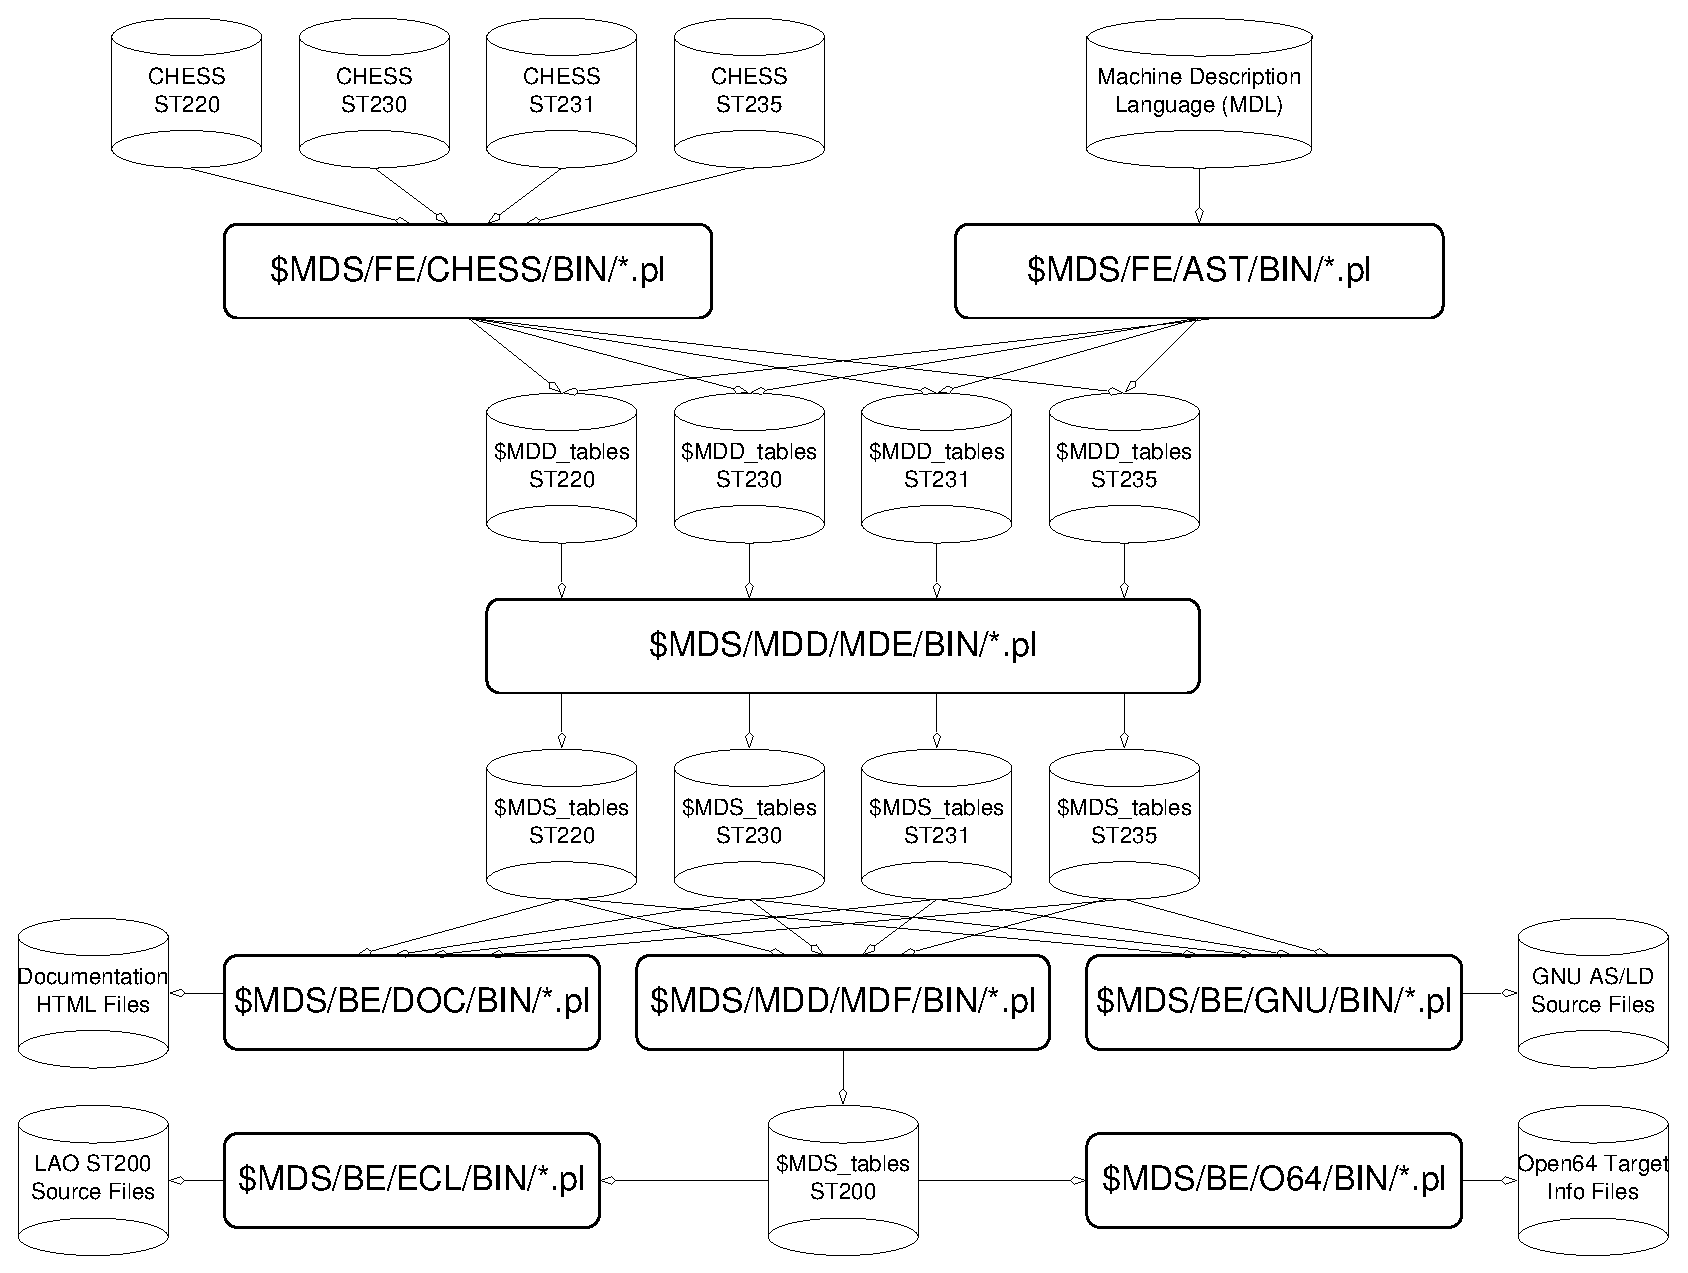
\epsfig{file=FIG/mds-flow.eps,width=120mm}
\end{center}
\caption{MDS components and information flow.}
\label{fig:mds-flow}
\end{figure}

A Machine Description System (MDS) is a structured data repository and a
collection of programs used to target software development tools to a particular
computing machine. These software development tools include instruction set
simulator, binary utilities, C compiler, libraries and debugger. As illustrated
in figure~\ref{fig:mds-flow}, a MDS comprises front-end tools that processes
machine description sources to create a Machine Description Database (MDD). A
MDS also comprises back-end tools that process the MDD contents and instantiate
template files that are then used to build the software development tools.
Because several back-end processing tools need to share particular views of the
MDD contents, these views are created once by a Machine Description Expanded
(MDE) contents. Unlike the MDD, the MDE contains redundancy, but is better suited
to the needs of the MDS back-end processing tools.  \medskip

The software development tools need to implement a number of machine-dependent
tasks: \begin{description}

\item[Encoding and Decoding] The binary files that represent a target machine
program are encoded by the assembler and the linker, then decoded by the
simulator or the debugger.

\item[Assembling and Linking] The assembler needs to parse the assembly language
syntax in order to produce relocatable binary programs. The linker needs to
process the relocations in order to produce the executable binary programs. Both
the assembly language syntax and the relocation algorithms are
machine-dependent.

\item[Instruction Bundling] On a VLIW processor, the instructions are grouped
into bundles that execute in parallel. The instruction bundling constraints are
usually less regular that the instruction scheduling constraints. In particular,
the allowed contents of a bundle may be dependent on the bundle start address.
In case of the ST200, instruction bundling has to manage the operands with
immediate extensions.

\item[Instruction Simulation] The instruction simulator executes a target
machine program on a host machine and provides performance estimates. It needs
to model the behavior of the machine at the architecture level and the
cycle-accurate level.

\item[Instruction Scheduling] The compiler optimizes the target machine program
by reordering its operations order. In order to preform this scheduling, the
compiler needs an abstract model of the machine resources and of the dependence
latencies.

\item[Register Allocation] The register allocation of the compiler maps each
program variable to either target processor registers or to memory locations. To
make these decisions, the compiler needs a complete description of the registers
including the cost of moving their contents from / to memory.

\item[Operand Constraints] When optimizing the target machine program, the
compiler must satisfy the architecture constraints on the instruction operands.
In addition to a list of allowed registers, these include the kind of constants
available. An added difficulty for the compiler is to manage constraints on
operands that both read and write a register, such as with auto-modified
addressing modes.

\item[Instruction Rewriting] In this optimization, the compiler matches a
pattern of target machine operations and replaces it by a more effective
pattern. In its simplest form this is the so-called peephole optimization
(patterns are sequences). In the modern form, patterns are identified on the
data-flow graph and matching is enabled by predicates on the pattern operands
(such as the active bit width).

\item[Instruction Semantics] For the purposes of program analysis and
optimizations, the compiler needs the abstracted behaviors of the instructions.
The simplest example is constant propagation, where the compiler emulates the
target processor execution to reduce constant expressions. While behaviors are
usually expressed in an imperative programming language (such as a C subset),
instruction semantics are better expressed in an applicative language (no state)
and abstract the complex parts of behaviors such as exception detection.

\item[Instruction Attributes] Summary information about the instruction
properties are needed by the compiler optimizations, such as: control
instruction, memory access instruction, arithmetic instruction, arithmetic
properties, input and output precision, etc.

\item[Instruction Selection] The compiler must translate the machine-independent
expressions and statements into the target processor instructions. This is
usually done by minimum-cost covering of the expressions by tree patterns, where
each tree pattern represents a machine instruction.

\end{description}


\subsection{Design Requirements}

\begin{enumerate}

\item The MDD should overcome the restrictions of CHESS and MachGen.

\item The MDD should be able to replace the CHESS database.

\item The MDS should be able to replace the MachGen generators.

\item The MDS should configure the GNU assembler, linker and binary utilities.

\item The MDS should generate most of the Open64 target processor description.

\item The MDS should generate all the LAO target processor description.

\item The MDD should be able to represent complex architectures like the ARM.

\item The MDD should be able to represent ST200 SIMD architecture extensions.

\item The MDD schema should be non-redundant and pseudo-relational.

\item The MDS processing should only depend on open-source tools.

\item The MDS specifications and documentation should be open.

\item The MDD representation should be valid XML documents.

\end{enumerate}

The most critical design decision is the schema of the MDD. An machine
description is most efficiently specified by a set of related tables, as
illustrated by a typical processor architecture manual and also by the tables
of the CHESS database (one table per \texttt{.db} file). This motivates the
requirement that the MDD schema be pseudo-relational. Pseudo-relational means
that the database is not in first normal form (1NF), that is, it allows list to
be contained in some of the attributes. Other relational normalizations should
apply to remove redundancy. \medskip

The requirement to represent the MDD in XML is motivated by the fact that the
MDD contents should be in text form, in order to facilitate the all-important
revision tracking.  Since the MDD contents is structured, the natural choice is
to use XML for the representation. Thanks to XML, the low-level aspects of text
file processing such as inclusion, macro expansion, Unicode escape sequence
encoding are readily available from many tools and libraries. The XML
representation also to validate a structured in a document content against a
schema. Last, the processing of XML into user-facing documentation can be
completely automated with already existing tools. \medskip

The requirement that the MDD is represented by valid XML documents has a precise
meaning. The W3C Extensible Markup Language (XML) 1.0 recommendation specifies
how the Document Type Definition (DTD) defines the schema of any XML document
for the purposes of validation. In particular, the validity of cross-references
between elements of a XML document can only checked by a validating parser if
the element attributes are declared as ID and IDREF or IDREFS in the document
DTD. While using alternate XML schema definition languages\footnote{XML Schema
from W3C and RelaxNG from OASIS.} enables a better validation of the XML
documents, these languages are outside of the XML specification and are still
being defined. For these reasons, the schema of the MDD contents should be
expressed by a DTD.

\section{The Machine Description Database Schema}

\subsection{Database Schema Design Guidelines}

The Machine Description Database (MDD) schema is specified with commented
fragments of the MDD DTD. For the definition of the XML elements, we apply the
following guidelines: \begin{itemize}

\item Keep the tuple form of relational tables where possible. This implies that
most elements have empty content.

\item Represent list of ELEMENT references as IDREFS attribute values. This
allow to keep the tuple form while avoiding the proliferation of auxiliary
markup. The XML validation ensures that IDREF and IDREFS attributes are not
dangling.

\item When using IDREFS attribute values, make sure that the elements referenced
are all of the same type. This eases the representation of the MDD contents in
processing tools, as elements map to objects and IDREF become object pointers.

\item Likewise, represent list of values as white-space separated tokens in
NMTOKENS attributes. A SGML NMTOKEN matches names and numbers without '+'
characters.

\end{itemize} 

Some MDD elements have a \texttt{name} attribute that is later used to construct
other \texttt{name} or \texttt{ID} attributes. These attributes have an inner
sequence structure that can be recovered by splitting around ':' characters.

\input MDD.latex


\section{Behavior and Semantics in the MDS}

\subsection{Design of the Behavior and Semantics Languages}

The MDS specifies Behavior for the Instruction(s) and Semantics for the
Operator(s). The Behavior and Semantics specifications are available in a
textual language that is a straightforward representation of the corresponding
abstract syntax trees. These languages have been designed under the following
requirements: \begin{itemize}

\item The Behavior language should enable the generation of behavioral code for
instruction simulators.

\item The Semantics language should be able to represent the effects of native
instructions and intrinsic operators for the purpose of code selection.

\item There should exist a clear process for generating the Semantics from the
Behavior of any instruction.

\end{itemize}

After reviewing several systems for behavior and semantics representation,
(including the LCC node operators, the LLVM instruction set, the Open64 WHIRL
specification, the CSDL RTL specifications, Christophe Guillon's TTL / RTL
languages, we adopted the following design: \begin{itemize}

\item The Behavior language is based on statements and captures common
sub-expressions in temporary variables. It has control-flow constructs but no
looping nor recursion. Computations are carried with infinite precision
arithmetic.

\item The Semantics language is a parallel list of guarded computations, where
each computation is either a \texttt{STORE} to a variable or a memory access or
a \texttt{THROW} of an exception. There are no common sub-expressions between
the commands, as all occurrences of temporary variables are forward-substituted.
All computations are annotated with the machine type, which included the minimum
bit precision required for correctness.

\end{itemize}


\subsection{Behavior Grammar Specification}

\subsection{Semantics Grammar Specification}


\section{Design Notes}


\subsection{Design Orientations}

\begin{itemize}

\item The MDS should flatten information even if input was given in a structured
way, then reconstruct its own hierarchies bottom up. For instance: Decoding
trees, Bundling classes, Operator Semantics, Operator Selection.

\item Aliasing between storage elements must be properly handled. This includes
aliasing control registers like PC or PSW with memory, data registers with
control registers and data registers from different RegClass(es).

\item The Instruction have a Behavior derived from Takumi or PseudoC. The
instruction Opcode(s) specialize this Behavior with respect to Storage Access.
The Operator build procedures convert the Opcode Behavior into Semantics. Then
the Semantics is abstracted into Selection by filtering out LOADs and STOREs to
Register Storage.

\end{itemize}


\subsection{Comparison with CHESS}

The specific problems identified with CHESS are: \begin{itemize}

\item CHESS has no concept of instruction modifier (see Modifier in
\S\ref{sec:Modifier}). On the ST200, the dismissible bit is a modifier and more
modifiers are expected with SIMD architecture extensions. Using modifiers enable
further reduction of an architecture description.

\item CHESS defines an operand as a bit-field augmented with a \texttt{kind}
flag that is either \texttt{src} or \texttt{dst}, as defined by
\texttt{st230/fld.db}. In fact, an operand (see Operand in \S\ref{sec:Operand})
is a higher-level construct that may contain a register reference an immediate
or a modifier. The register reference can be used for both reading and writing,
for instance in case of auto-modified addressing modes.

\item In case of Immediate operand, CHESS does not distinguish between the
encoding of an immediate value in a field and the value itself and it omits the
immediate sign extension.

\item In case of RegClass operand, CHESS does not distinguish between the
destination registers r0..r63 and the destination registers r0..r62.

\end{itemize}

On the other hand, the CHESS database contains the most structured specification
of the ST200 available today. This is the reason we populate the contents of our
prototype MDD by scripting the CHESS database contents.


\subsection{Comparison with MachGen}

\begin{itemize}

\item MachGen Modifier is contained in Format, not in Operand

\item MachGen has no reserved BitField(s). By default the unspecified bits in a
Format are assumed reserved and are cleared.

\end{itemize}

\subsection{Comparison with Open64}

\begin{itemize}

\item Open64 Register Class $\rightarrow$ MDS Storage with register kind.

\item Open64 Register SubClass $\rightarrow$ MDS RegClass.

\item A read-write Operand translate to one Open64 Operand and one Result
connected by Same\_Res.

\end{itemize}


\end{document}

